\chapter{System Design}

This chapter presents the complete system design of ZeroAuth through standard engineering diagrams including the system architecture, use case diagram, data flow diagrams, sequence diagram, flowcharts, block diagram, and database schema. Each diagram is accompanied by a detailed explanation of the design decisions and data flows it represents.

% ═══════════════════════════════════════════════════════════════
\section{System Architecture Diagram}

\noindent\begin{minipage}{\linewidth}
\centering
\begin{tikzpicture}[node distance=1.0cm,
    box/.style={draw, rounded corners, fill=#1, minimum width=3cm,
                minimum height=0.72cm, text centered, font=\small},
    arr/.style={->, >=stealth, thick}]

  % === VERIFIER (col 1) ===
  \node[box=orange!20] (sdk)    {ZeroAuth SDK};
  \node[box=orange!20, below=0.5cm of sdk] (qrdisp) {QR Display};
  \node[draw, dashed, rounded corners, fit=(sdk)(qrdisp), inner sep=0.3cm,
        label=above:{\textbf{Verifier Website}}] (vbox){};

  % === RELAY (col 2) ===
  \node[box=green!20,  right=3.2cm of sdk]  (api)  {Express.js API};
  \node[box=green!20,  below=0.4cm of api]  (val)  {Validation Layer};
  \node[box=green!20,  below=0.4cm of val]  (zkv)  {ZK Verifier (snarkjs)};
  \node[box=green!20,  below=0.4cm of zkv]  (db)   {Supabase (PostgreSQL)};
  \node[draw, dashed, rounded corners, fit=(api)(val)(zkv)(db), inner sep=0.3cm,
        label=above:{\textbf{Relay Server}}] (rbox){};

  % === WALLET (col 3) ===
  \node[box=blue!15,  right=3.2cm of api] (ui)  {React Native UI};
  \node[box=blue!15,  below=0.4cm of ui]  (qrs) {QR Scanner};
  \node[box=blue!15,  below=0.4cm of qrs] (pg)  {ZK Proof Engine};
  \node[box=blue!15,  below=0.4cm of pg]  (wm)  {Wallet (Ed25519)};
  \node[draw, dashed, rounded corners, fit=(ui)(qrs)(pg)(wm), inner sep=0.3cm,
        label=above:{\textbf{Mobile Wallet}}] (wbox){};

  % === ARROWS ===
  \draw[arr] (sdk.east)   -- node[above,font=\footnotesize]{① Create Session} (api.west);
  \draw[arr] (wm.west)    -- node[below,font=\footnotesize]{⑤ Submit Proof}   (db.east);
  \draw[arr,<->] (api)--(val);
  \draw[arr]     (val)--(zkv);
  \draw[arr,<->] (zkv)--(db);
  \draw[arr]     (qrs)--(pg);
  \draw[arr]     (pg)--(wm);
  \draw[arr, dashed] (qrdisp.east) -- ++(0.6,0) |-
        node[near start, above, font=\footnotesize]{④ QR Scan} (qrs.west);
\end{tikzpicture}
\captionof{figure}{System Architecture Diagram}
\label{fig:architecture}
\end{minipage}

\vspace{0.4cm}
The ZeroAuth system is composed of three primary components connected through secure HTTPS channels. The Verifier Website embeds the ZeroAuth JavaScript SDK, which sends a session creation request to the Relay API (step 1) and renders the received QR payload as a scannable code on screen. The Relay Server acts as the central processing hub, where the Express.js API receives requests, passes them through a Validation Layer for schema and session integrity checks, and then forwards the proof data to the ZK Verifier powered by snarkjs. All session data and verification keys are persisted in Supabase PostgreSQL. The Mobile Wallet, implemented in React Native, scans the displayed QR code (step 4) using the device camera, identifies the matching credential, generates a Groth16 zero-knowledge proof through the ZK Engine, and submits it back to the Relay (step 5). Critically, no private credential data ever leaves the device -- only the cryptographic proof and its public signals are transmitted across the network.

% ═══════════════════════════════════════════════════════════════
\newpage
\section{Use Case Diagram}

\noindent\begin{minipage}{\linewidth}
\centering
\begin{tikzpicture}[scale=0.80, every node/.style={scale=0.80}]

  % --- Actor: Wallet User ---
  \node[draw, circle, fill=black, minimum size=0.28cm] (uh) at (-5.5, 4.8) {};
  \draw (-5.5,4.52) -- (-5.5,3.9);
  \draw (-5.8,4.3) -- (-5.2,4.3);
  \draw (-5.5,3.9) -- (-5.8,3.5);
  \draw (-5.5,3.9) -- (-5.2,3.5);
  \node[font=\small, below=1.4cm of uh] {\textbf{Wallet User}};

  % --- Actor: Verifier ---
  \node[draw, circle, fill=black, minimum size=0.28cm] (vh) at (5.8, 4.8) {};
  \draw (5.8,4.52) -- (5.8,3.9);
  \draw (5.5,4.3) -- (6.1,4.3);
  \draw (5.8,3.9) -- (5.5,3.5);
  \draw (5.8,3.9) -- (6.1,3.5);
  \node[font=\small, below=1.4cm of vh] {\textbf{Verifier}};

  % --- Actor: Relay Server ---
  \node[draw, circle, fill=black, minimum size=0.28cm] (rh) at (5.8, 0.2) {};
  \draw (5.8,-0.08) -- (5.8,-0.7);
  \draw (5.5,-0.3) -- (6.1,-0.3);
  \draw (5.8,-0.7) -- (5.5,-1.1);
  \draw (5.8,-0.7) -- (6.1,-1.1);
  \node[font=\small, below=1.4cm of rh] {\textbf{Relay Server}};

  % Use cases
  \node[ellipse, draw, fill=blue!8, minimum width=3.4cm, minimum height=0.7cm,
        text centered, font=\small] (u1) at (0, 4.8) {Add Credential};
  \node[ellipse, draw, fill=blue!8, minimum width=3.4cm, minimum height=0.7cm,
        text centered, font=\small] (u2) at (0, 3.5) {Scan QR Code};
  \node[ellipse, draw, fill=blue!8, minimum width=3.4cm, minimum height=0.7cm,
        text centered, font=\small] (u3) at (0, 2.2) {Generate ZK Proof};
  \node[ellipse, draw, fill=blue!8, minimum width=3.4cm, minimum height=0.7cm,
        text centered, font=\small] (u4) at (0, 0.9) {Approve Request};
  \node[ellipse, draw, fill=blue!8, minimum width=3.4cm, minimum height=0.7cm,
        text centered, font=\small] (u5) at (0,-0.4) {View Sessions};
  \node[ellipse, draw, fill=blue!8, minimum width=3.4cm, minimum height=0.7cm,
        text centered, font=\small] (u6) at (0,-1.7) {Set / Verify PIN};

  \node[ellipse, draw, fill=orange!12, minimum width=3.2cm, minimum height=0.7cm,
        text centered, font=\small] (v1) at (0, 6.1) {Create Session};
  \node[ellipse, draw, fill=orange!12, minimum width=3.2cm, minimum height=0.7cm,
        text centered, font=\small] (v2) at (0, 7.4) {Display QR Code};

  \node[ellipse, draw, fill=green!12, minimum width=3.2cm, minimum height=0.7cm,
        text centered, font=\small] (r1) at (0,-3.0) {Verify ZK Proof};
  \node[ellipse, draw, fill=green!12, minimum width=3.2cm, minimum height=0.7cm,
        text centered, font=\small] (r2) at (0,-4.3) {Manage Sessions};

  % Connections
  \foreach \x in {u1,u2,u3,u4,u5,u6} \draw (-5.5,4.0) -- (\x);
  \foreach \x in {v1,v2}              \draw (5.8,4.0)  -- (\x);
  \foreach \x in {r1,r2}              \draw (5.8,0.0)  -- (\x);

  \draw[dashed,->,>=stealth] (u2) -- node[right,font=\scriptsize]{$\langle\langle$includes$\rangle\rangle$}(u3);
  \draw[dashed,->,>=stealth] (u3) -- node[right,font=\scriptsize]{$\langle\langle$includes$\rangle\rangle$}(u4);

  \node[draw, dashed, rounded corners,
        fit=(u1)(u2)(u3)(u4)(u5)(u6)(v1)(v2)(r1)(r2),
        inner sep=0.5cm, label=above:{\textbf{ZeroAuth System}}]{};
\end{tikzpicture}
\captionof{figure}{Use Case Diagram}
\label{fig:usecase}
\end{minipage}

\vspace{0.4cm}
Three actors interact with the ZeroAuth system. The Wallet User has six primary use cases: adding credentials to the local wallet, scanning verifier QR codes, generating ZK proofs, approving verification requests, viewing session history, and setting or verifying their device PIN. The Verifier actor, representing any third-party website using the SDK, creates verification sessions and displays QR codes. The Relay Server actor handles proof verification and manages the session lifecycle between PENDING and COMPLETED states. The $\langle\langle$includes$\rangle\rangle$ relationships between Scan QR Code, Generate ZK Proof, and Approve Request indicate that these steps are automatically chained together whenever the user initiates a scan.

% ═══════════════════════════════════════════════════════════════
\newpage
\section{Data Flow Diagram -- Level 0 (Context Diagram)}

\noindent\begin{minipage}{\linewidth}
\centering
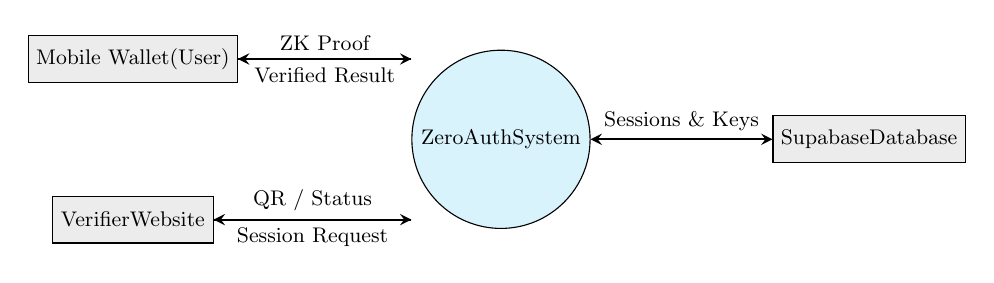
\begin{tikzpicture}[scale=0.85, every node/.style={scale=0.85},
    ext/.style={rectangle, draw, fill=gray!15, minimum width=2.4cm,
                minimum height=0.7cm, text centered, font=\small},
    proc/.style={circle, draw, fill=cyan!15, minimum size=2.6cm,
                 text centered, font=\small},
    arr/.style={->,>=stealth,thick}]

  \node[proc]  (sys)    at (0,0)    {ZeroAuth\\System};
  \node[ext]   (wallet) at (-5.5, 1.2) {Mobile Wallet\\(User)};
  \node[ext]   (web)    at (-5.5,-1.2) {Verifier\\Website};
  \node[ext]   (db)     at ( 5.5, 0)   {Supabase\\Database};

  \draw[arr] (wallet.east) -- node[above,font=\small]{ZK Proof} (sys.west |- wallet);
  \draw[arr] (sys.west |- wallet) -- node[below,font=\small]{Verified Result} (wallet.east);
  \draw[arr] (web.east) -- node[below,font=\small]{Session Request} (sys.west |- web);
  \draw[arr] (sys.west |- web) -- node[above,font=\small]{QR / Status} (web.east);
  \draw[arr,<->] (sys) -- node[above,font=\small]{Sessions \& Keys} (db);
\end{tikzpicture}
\captionof{figure}{DFD Level 0 -- Context Diagram}
\label{fig:dfd0}
\end{minipage}

\vspace{0.3cm}
The context diagram treats the entire ZeroAuth system as a single black-box process. The Mobile Wallet submits a Zero-Knowledge Proof and receives a verified result. The Verifier Website sends a session creation request and receives a QR payload and status updates. The Supabase Database provides bidirectional storage for sessions and verification keys.

\vspace{0.4cm}

% ─────────────────────────────────────────────────────────────
\subsection{DFD Level 1 -- Internal Processes}

\noindent\begin{minipage}{\linewidth}
\centering
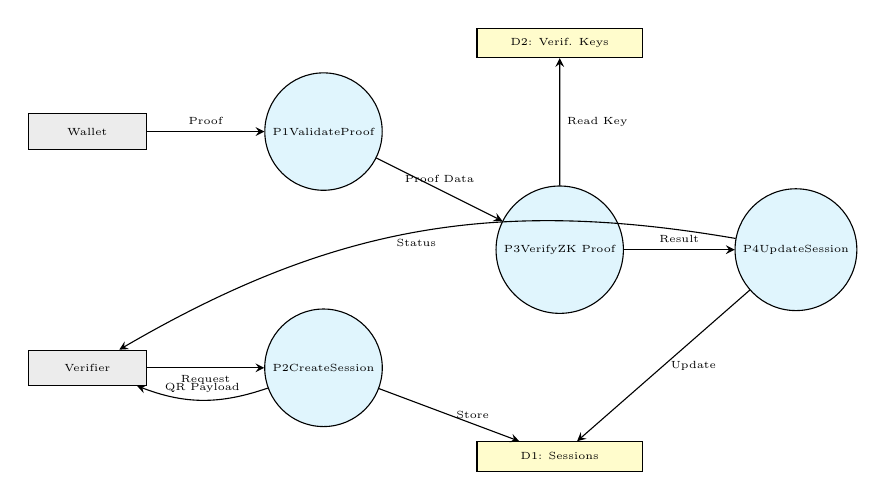
\begin{tikzpicture}[scale=0.75, every node/.style={scale=0.75},
    proc/.style={circle, draw, fill=cyan!12, minimum size=1.6cm,
                 text centered, font=\tiny},
    store/.style={rectangle, draw, fill=yellow!20, minimum width=2.8cm,
                  minimum height=0.5cm, text centered, font=\tiny},
    ext/.style={rectangle, draw, fill=gray!15, minimum width=2cm,
                minimum height=0.6cm, text centered, font=\tiny},
    arr/.style={->,>=stealth}]

  \node[ext]   (wallet) at (-6, 2)   {Wallet};
  \node[ext]   (web)    at (-6,-2)   {Verifier};
  \node[proc]  (p1)     at (-2, 2)   {P1\\Validate\\Proof};
  \node[proc]  (p2)     at (-2,-2)   {P2\\Create\\Session};
  \node[proc]  (p3)     at ( 2, 0)   {P3\\Verify\\ZK Proof};
  \node[proc]  (p4)     at ( 6, 0)   {P4\\Update\\Session};
  \node[store] (ds1)    at ( 2,-3.5) {D1: Sessions};
  \node[store] (ds2)    at ( 2, 3.5) {D2: Verif. Keys};

  \draw[arr] (wallet)--(p1) node[midway,above,font=\tiny]{Proof};
  \draw[arr] (web)--(p2)   node[midway,below,font=\tiny]{Request};
  \draw[arr] (p1)--(p3)   node[midway,above,font=\tiny]{Proof Data};
  \draw[arr] (p2)--(ds1)  node[midway,right,font=\tiny]{Store};
  \draw[arr] (p3)--(ds2)  node[midway,right,font=\tiny]{Read Key};
  \draw[arr] (p3)--(p4)   node[midway,above,font=\tiny]{Result};
  \draw[arr] (p4)--(ds1)  node[midway,right,font=\tiny]{Update};
  \draw[arr] (p4) to [bend right=20] node[below,font=\tiny]{Status} (web);
  \draw[arr] (p2) to [bend left=20]  node[above,font=\tiny]{QR Payload} (web);
\end{tikzpicture}
\captionof{figure}{DFD Level 1 -- Internal Processes}
\label{fig:dfd1}
\end{minipage}

\vspace{0.4cm}
The Level 1 DFD decomposes the system into four internal processes. Process P1 validates the structure and schema of incoming proof submissions from the Wallet, checking that all required fields are present and correctly formatted. Process P2 handles session creation requests from the Verifier, stores the new session record in data store D1, and returns a QR payload. Process P3 reads the appropriate Groth16 verification key from data store D2 and cryptographically verifies the submitted proof using snarkjs. Process P4 updates the session status in D1 to COMPLETED upon successful verification and sends the final result back to the Verifier.

% ═══════════════════════════════════════════════════════════════
\newpage
\section{Sequence Diagram}

\noindent\begin{minipage}{\linewidth}
\centering
\begin{tikzpicture}[scale=0.75, every node/.style={scale=0.75},
    life/.style={draw, fill=white, minimum width=1.5cm,
                 minimum height=0.5cm, text centered, font=\small\bfseries},
    msg/.style={->, >=stealth, font=\scriptsize}]

  \node[life, fill=orange!20] (W) at (0,  0) {Verifier};
  \node[life, fill=green!20]  (R) at (4,  0) {Relay};
  \node[life, fill=blue!15]   (M) at (8,  0) {Wallet};
  \node[life, fill=gray!15]   (D) at (12, 0) {Supabase};

  \foreach \x in {0,4,8,12}
    \draw[dashed, gray] (\x,-0.3) -- (\x,-11);

  \draw[msg] (0,-1.0) -- (4,-1.0)  node[midway,above]{① POST /sessions (credType)};
  \draw[msg] (4,-1.7) -- (12,-1.7) node[midway,above]{② INSERT session row};
  \draw[msg] (12,-2.4)-- (4,-2.4)  node[midway,above]{③ session\_id + nonce};
  \draw[msg] (4,-3.1) -- (0,-3.1)  node[midway,above]{④ QR payload (Base64)};
  \draw[msg] (0,-3.8) -- (8,-3.8)  node[midway,above]{⑤ Scan QR (camera)};
  \draw[->,>=stealth,font=\scriptsize,looseness=5]
        (8,-4.6) to [out=30,in=-30] node[right]{⑥ groth16.fullProve()} (8,-5.8);
  \draw[msg] (8,-6.5) -- (4,-6.5)  node[midway,above]{⑦ POST /sessions/:id/proof};
  \draw[msg] (4,-7.2) -- (12,-7.2) node[midway,above]{⑧ SELECT key\_data};
  \draw[msg] (12,-7.9)-- (4,-7.9)  node[midway,above]{⑨ verification key JSON};
  \node[font=\scriptsize,align=center] at (4.8,-8.6) {⑩ snarkjs.groth16.verify()};
  \draw[msg] (4,-9.3) -- (12,-9.3) node[midway,above]{⑪ UPDATE status=COMPLETED};
  \draw[msg] (4,-10.0)-- (8,-10.0) node[midway,above]{⑫ 200 OK};
  \draw[msg] (0,-10.6)-- (4,-10.6) node[midway,above]{⑬ GET /sessions/:id (poll)};
  \draw[msg] (4,-11.2)-- (0,-11.2) node[midway,above]{⑭ \{status: COMPLETED\}};
\end{tikzpicture}
\captionof{figure}{Sequence Diagram -- Verification Flow}
\label{fig:sequence}
\end{minipage}

\vspace{0.4cm}
The sequence diagram shows the full temporal interaction between the four system participants. The Verifier initiates the flow by posting a session creation request to the Relay (step 1), which stores the session in Supabase (step 2) and returns a session ID and nonce (step 3) encoded into a QR payload (step 4). The Wallet scans the QR code (step 5) and internally runs \texttt{groth16.fullProve()} to generate a cryptographic proof (step 6), which is then submitted to the Relay (step 7). The Relay retrieves the corresponding verification key from the database (steps 8--9), verifies the proof using snarkjs (step 10), and upon success updates the session status to COMPLETED in Supabase (step 11) before returning a 200 OK to the Wallet (step 12). The Verifier detects the completion through periodic polling (steps 13--14) and grants access to the authenticated user.

% ═══════════════════════════════════════════════════════════════
\newpage
\section{Flowchart -- Overall Verification Flow}

\noindent\begin{minipage}{\linewidth}
\centering
\begin{tikzpicture}[node distance=0.55cm, scale=0.58, every node/.style={scale=0.58},
    slim/.style={process, minimum width=4.5cm, minimum height=0.55cm, font=\small}]

  \node[startstop]  (s0) {Start};
  \node[slim, below=of s0]  (p1) {Verifier loads ZeroAuth SDK};
  \node[slim, below=of p1]  (p2) {SDK creates session on Relay};
  \node[slim, below=of p2]  (p3) {Relay returns QR payload};
  \node[slim, below=of p3]  (p4) {SDK renders QR code};
  \node[slim, below=of p4]  (p5) {User scans QR with Wallet};
  \node[decision, below=of p5, aspect=3, font=\small] (d1) {Valid QR?};
  \node[slim, right=1.8cm of d1, fill=red!15]  (e1) {Show Error};
  \node[decision, below=0.9cm of d1, aspect=3, font=\small] (d2) {Credential match?};
  \node[slim, right=1.8cm of d2, fill=red!15]  (e2) {No Match};
  \node[slim, below=0.9cm of d2]  (p6) {User approves request};
  \node[slim, below=of p6]  (p7) {Generate ZK Proof};
  \node[slim, below=of p7]  (p8) {Submit proof to Relay};
  \node[decision, below=of p8, aspect=3, font=\small] (d3) {ZK Valid?};
  \node[slim, right=1.8cm of d3, fill=red!15]  (e3) {Reject Proof};
  \node[slim, below=0.9cm of d3]  (p9) {Session COMPLETED};
  \node[slim, below=of p9]  (p10){SDK detects via polling};
  \node[startstop, below=of p10, fill=green!20] (s1) {Access Granted};

  \draw[arrow] (s0)--(p1)--(p2)--(p3)--(p4)--(p5)--(d1);
  \draw[arrow] (d1)--node[above,font=\scriptsize]{No} (e1);
  \draw[arrow] (d1)--node[left, font=\scriptsize]{Yes}(d2);
  \draw[arrow] (d2)--node[above,font=\scriptsize]{No} (e2);
  \draw[arrow] (d2)--node[left, font=\scriptsize]{Yes}(p6);
  \draw[arrow] (p6)--(p7)--(p8)--(d3);
  \draw[arrow] (d3)--node[above,font=\scriptsize]{No} (e3);
  \draw[arrow] (d3)--node[left, font=\scriptsize]{Yes}(p9)--(p10)--(s1);
\end{tikzpicture}
\captionof{figure}{Overall Verification Flowchart}
\label{fig:flowchart_main}
\end{minipage}

\vspace{0.3cm}
The overall verification flowchart captures the complete decision logic from session initiation to access grant. The Verifier website loads the SDK, which creates a session on the Relay and receives a QR payload that is rendered for the user. When the Wallet scans the QR code, the system first checks if the QR is valid and not expired. If valid, it checks whether the user has a credential that matches the requested type. On a successful credential match and user approval, the ZK proof is generated locally and submitted to the Relay. The Relay then performs cryptographic verification using snarkjs; an invalid proof is rejected immediately. On success, the session is marked COMPLETED, the SDK detects this via periodic polling, and the Verifier website grants access to the user. All failure paths terminate the flow early without any sensitive data disclosure.

% ═══════════════════════════════════════════════════════════════
\newpage
\section{ZK Proof Generation Flowchart}

\noindent\begin{minipage}{\linewidth}
\centering
\begin{tikzpicture}[node distance=0.8cm, scale=0.65, every node/.style={scale=0.65}]
  \node[startstop] (s0) {Proof Generation Triggered};
  \node[process, below=of s0]   (p1) {Validate credential expiry};
  \node[decision, below=of p1, aspect=2.5]  (d1) {Expired?};
  \node[startstop, right=2.6cm of d1, fill=red!25] (e1) {Error: Expired};
  \node[decision, below=1.1cm of d1, aspect=2.5]  (d2) {Assets cached?};
  \node[process, right=2.6cm of d2] (p2) {Download WASM + zkey};
  \node[process, below=1.1cm of d2] (p3) {Load from cache};
  \node[process, below=of p3]  (p4) {Prepare circuit inputs};
  \node[process, below=of p4]  (p5) {WebView: groth16.fullProve()};
  \node[decision, below=of p5, aspect=2.5]  (d3) {Done in 90s?};
  \node[startstop, right=2.6cm of d3, fill=red!25] (e2) {Timeout Error};
  \node[startstop, below=1.1cm of d3, fill=green!20] (s1) {ZKProofPayload};

  \draw[arrow] (s0)--(p1)--(d1);
  \draw[arrow] (d1)--node[above]{Yes}(e1);
  \draw[arrow] (d1)--node[left]{No}(d2);
  \draw[arrow] (d2)--node[above]{No}(p2);
  \draw[arrow] (d2)--node[left]{Yes}(p3);
  \draw[arrow] (p2)|-(p4);
  \draw[arrow] (p3)--(p4)--(p5)--(d3);
  \draw[arrow] (d3)--node[above]{No}(e2);
  \draw[arrow] (d3)--node[left]{Yes}(s1);
\end{tikzpicture}
\captionof{figure}{ZK Proof Generation Flowchart}
\label{fig:flowchart_zk}
\end{minipage}

\vspace{0.4cm}
This flowchart details the internal proof generation process within the mobile Wallet. The process begins by validating whether the selected credential has expired, immediately terminating with an error if it has. Next, the system checks whether the WASM circuit file and zkey file are cached locally from a previous run. If not cached, they are downloaded from the bundled assets and stored for future use. The circuit inputs, which include values such as the birth year, random salt, current year, and minimum age threshold, are then prepared and passed to a sandboxed WebView bridge which executes \texttt{snarkjs.groth16.fullProve()}. A 90-second timeout is enforced to accommodate low-end devices. On successful completion within the time limit, a ZKProofPayload containing the proof elements $\pi_a$, $\pi_b$, $\pi_c$ and the public signals is returned for submission to the Relay.

% ═══════════════════════════════════════════════════════════════
\newpage
\section{Block Diagram}

\noindent\begin{minipage}{\linewidth}
\centering
\begin{tikzpicture}[node distance=0.5cm, scale=0.65, every node/.style={scale=0.65},
    blk/.style={draw, rounded corners, fill=#1, minimum width=2.0cm,
                minimum height=0.6cm, text centered, font=\small}]

  \node[blk=blue!20] (usr)  {User};
  \node[blk=blue!15, right=0.4cm of usr]  (cam)  {Camera};
  \node[blk=blue!15, right=0.4cm of cam]  (wapp) {Wallet App};
  \node[blk=blue!10, below=0.45cm of wapp] (crd) {Credential Store};
  \node[blk=blue!10, right=0.4cm of wapp] (zke)  {ZK Engine};
  \node[blk=blue!10, below=0.45cm of crd] (key)  {Ed25519 Keys};
  \node[draw,dashed,rounded corners,
        fit=(usr)(cam)(wapp)(crd)(zke)(key), inner sep=0.25cm,
        label=above:{\footnotesize\textbf{User Device}}]{};

  \node[blk=yellow!25, below=1.3cm of cam, minimum width=3.2cm] (net) {HTTPS / REST API};

  \node[blk=green!20, below=0.75cm of net] (rel) {Relay (Express.js)};
  \node[blk=green!15, left=0.4cm  of rel]  (zkv) {ZK Verifier};
  \node[blk=green!15, right=0.4cm of rel]  (sup) {Supabase DB};
  \node[draw,dashed,rounded corners,
        fit=(rel)(zkv)(sup), inner sep=0.25cm,
        label=below:{\footnotesize\textbf{Cloud Infrastructure}}]{};

  \draw[->,>=stealth] (usr)--(cam);
  \draw[->,>=stealth] (cam)--(wapp);
  \draw[<->,>=stealth] (wapp)--(crd);
  \draw[->,>=stealth] (wapp)--(zke);
  \draw[<->,>=stealth] (wapp)|-(net);
  \draw[<->,>=stealth] (net)--(rel);
  \draw[<->,>=stealth] (rel)--(zkv);
  \draw[<->,>=stealth] (rel)--(sup);
\end{tikzpicture}
\captionof{figure}{Block Diagram}
\label{fig:block}
\end{minipage}

\vspace{0.3cm}
The block diagram illustrates the physical and logical separation of the ZeroAuth system across two tiers. The User Device layer contains the Wallet application, which interfaces with the camera for QR scanning, the Credential Store for local data persistence, the ZK Engine for proof generation, and the Ed25519 key module for identity management. All proof-related communication between the device and the cloud is channelled exclusively through the HTTPS REST API layer, ensuring that no raw credential data crosses this boundary. The Cloud Infrastructure layer contains the Express.js Relay server, the snarkjs ZK Verifier component for cryptographic proof validation, and the Supabase PostgreSQL database for session and verification key storage.

\vspace{0.5cm}

% ─────────────────────────────────────────────────────────────
\section{Database Schema (ER Diagram)}

\noindent\begin{minipage}{\linewidth}
\centering
\begin{tikzpicture}[scale=0.72, every node/.style={scale=0.72}]
  \node[draw, fill=blue!10, minimum width=5.2cm, minimum height=0.7cm,
        text centered, font=\normalsize\bfseries] (st) at (0,0) {SESSIONS};
  \node[draw, below=0cm of st, minimum width=5.2cm, text width=4.8cm,
        font=\small, align=left] (sf) {
    \texttt{id}: UUID (PK)\\
    \texttt{session\_id}: TEXT (UNIQUE)\\
    \texttt{nonce}: TEXT\\
    \texttt{credential\_type}: TEXT \textrightarrow\ FK\\
    \texttt{status}: TEXT (PENDING/COMPLETED)\\
    \texttt{proof}: JSONB\\
    \texttt{proof\_hash}: TEXT\\
    \texttt{expires\_at}: TIMESTAMPTZ
  };

  \node[draw, fill=green!10, minimum width=5.2cm, minimum height=0.7cm,
        text centered, font=\normalsize\bfseries] (vt) at (8.5,0) {VERIFICATION\_KEYS};
  \node[draw, below=0cm of vt, minimum width=5.2cm, text width=4.8cm,
        font=\small, align=left] (vf) {
    \texttt{id}: UUID (PK)\\
    \texttt{credential\_type}: TEXT (UNIQUE)\\
    \texttt{key\_data}: JSONB\\
    \texttt{created\_at}: TIMESTAMPTZ
  };

  \draw[->,>=stealth,thick]
    ([yshift=0.5cm]sf.east) --
    node[above,font=\small]{references}
    ([yshift=0.5cm]vf.west);
\end{tikzpicture}
\captionof{figure}{Database ER Diagram}
\label{fig:er}
\end{minipage}

\vspace{0.3cm}
The database schema consists of two tables managed within Supabase PostgreSQL, both protected by Row-Level Security policies that restrict access exclusively to the Relay service role. The SESSIONS table records every verification request, storing the unique session identifier, a cryptographic nonce to prevent replay attacks, the credential type requested, the current session status (PENDING or COMPLETED), the submitted ZK proof in JSONB format, a SHA-256 hash of the proof for deduplication, and the session expiry timestamp. The VERIFICATION\_KEYS table holds the Groth16 verification key for each supported credential type as a JSONB object. The \texttt{credential\_type} field in SESSIONS acts as a foreign key reference to VERIFICATION\_KEYS, enabling the Relay to dynamically load the correct verification key at proof submission time without hardcoding per-circuit logic.
\end{minipage}
